\section{Database}
\subsection{Descrizione}
Per garantire la semplicità di gestione e la velocità di esecuzione delle query nel database sono presenti solo 3 tabelle: Users, Products e Transactions. Queste sono il minimo indispensabile per la creazione di un e-commerce funzionante. Quella riportata nel modello E/R è la prima versione del database che permette di caricare un'unica immagine per prodotto, nelle versioni successive verranno introdotti aggiornamenti graduali paralleli allo sviluppo completo del sito web. Il database è visualizzabile insieme a tutto il progetto scaricando la repository di GitHub \href{https://github.com/MauroPello/elaborato}{disponibile qui} \cite{GitHub}. 
\medskip

La tabella Users contiene le informazioni base necessarie per l'utilizzo della piattaforma: codice identificativo, nome utente, password, email identificativa, città di residenza, immagine di profilo, salt per la generazione dell'hash della password, api key per eseguire richieste tramite l'API e quantità di green coin posseduti. 
\medskip

La tabella Products contiene invece i seguenti campi: codice identificativo, nome, breve descrizione, immagine rappresentativa, disponibilità (per tenere traccia dei prodotti anche dopo la loro vendita o rimozione dal Marketplace), data dell'ultimo aggiornamento apportato e codice identificativo dell'utente proprietario del prodotto. 
\medskip

La tabella Transactions contiene le transazioni effettuate tra gli utenti descritte attraverso i seguenti campi: codice identificativo della transazione, codice identificativo del prodotto scambiato, codice identificativo dell'utente proprietario del prodotto al momento dello scambio (campo necessario per tenere traccia dei cambi di proprietà e delle transazioni anche dopo che queste si sono concluse), codice identificativo dell'utente acquirente, stato della transazione ("In Corso", "Completata Con Successo" o "Completata Senza Successo") e data dell'ultimo aggiornamento relativo alla transazione. 
\subsection{Modello E/R}
\begin{center}
    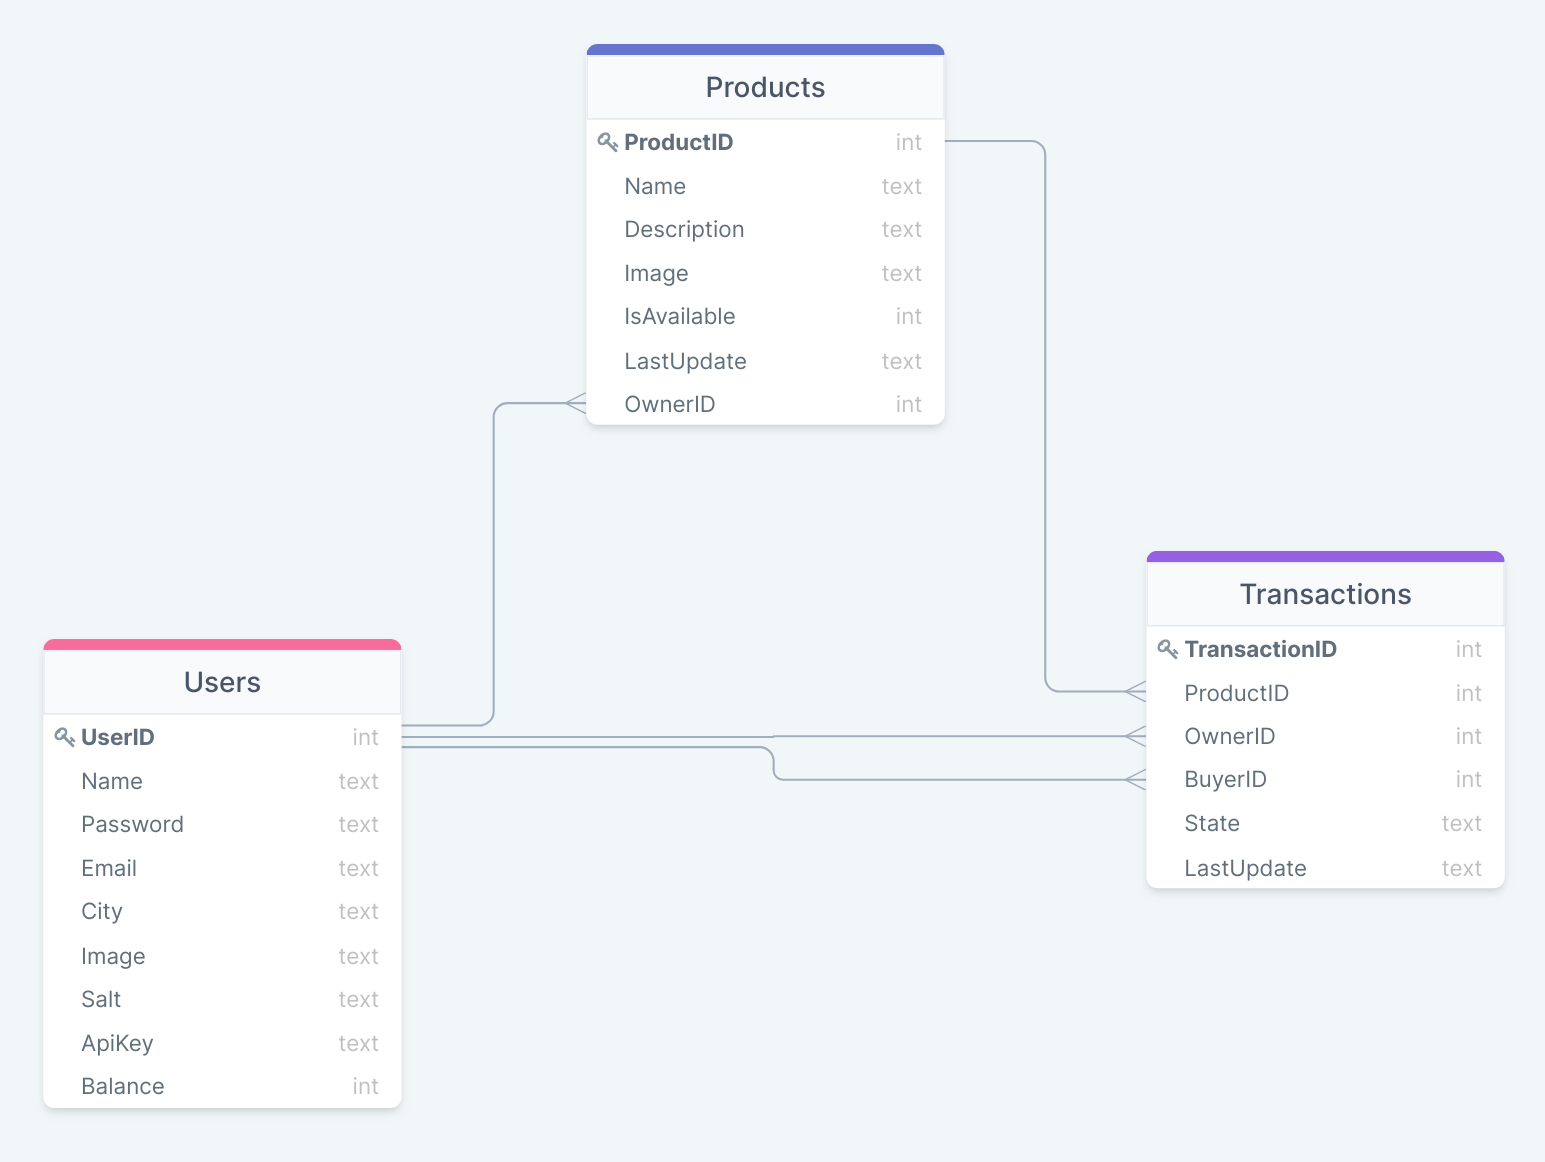
\includegraphics[scale=0.29]{images/modello_e_r.png}
\end{center}
\subsection{Modello logico}
\begin{center}
    \begin{tabular}{ |l|c|l| } 
    \hline
    \multicolumn{3}{|c|}{\large\textbf{Users}} \\
    \hline
    \textbf{Nome Campo} & \textbf{Tipo} & \textbf{Note} \\
    \hline
    UserID & INTEGER & NOT NULL, PK, AUTOINCREMENT \\
    Name & TEXT & NOT NULL \\
    Password & TEXT & NOT NULL \\
    Email & TEXT & NOT NULL \\
    City & TEXT & NOT NULL \\
    Image & TEXT & NOT NULL \\
    Salt & TEXT & NOT NULL \\
    ApiKey & TEXT & NOT NULL \\
    Balance & INTEGER & NOT NULL \\
    \hline
    \end{tabular}
\end{center}
\begin{center}
    \begin{tabular}{ |l|c|l| } 
    \hline
    \multicolumn{3}{|c|}{\large\textbf{Products}} \\
    \hline
    \textbf{Nome Campo} & \textbf{Tipo} & \textbf{Note} \\
    \hline
    ProductID & INTEGER & NOT NULL, PK, AUTOINCREMENT \\
    Name & TEXT & NOT NULL \\
    Description & TEXT & NOT NULL \\
    Image & TEXT & NOT NULL \\
    IsAvailable & INTEGER & NOT NULL \\
    LastUpdate & TEXT & NOT NULL \\
    OwnerID & INTEGER & NOT NULL, FK(Users) \\
    \hline
    \end{tabular}
\end{center}
\begin{center}
    \begin{tabular}{ |l|c|l| } 
    \hline
    \multicolumn{3}{|c|}{\large\textbf{Transactions}} \\
    \hline
    \textbf{Nome Campo} & \textbf{Tipo} & \textbf{Note} \\
    \hline
    TransactionID & INTEGER & NOT NULL, PK, AUTOINCREMENT \\
    ProductID & INTEGER & NOT NULL, FK(Products) \\
    OwnerID & INTEGER & NOT NULL, FK(Users) \\
    BuyerID & INTEGER & NOT NULL, FK(Users) \\
    State & TEXT & NOT NULL \\
    LastUpdate & TEXT & NOT NULL \\
    \hline
    \end{tabular}
\end{center}
\subsection{Entity Framework Core}
Il database è stato generato automaticamente da Entity Framework Core a partire dai modelli scritti in C\# e inseriti nel progetto (generazione code-first) \cite{EFcore}. I modelli inseriti devono essere riportati nel DbContext indicato nel file Startup.cs, il database context si occupa quindi di descrivere il database e le tabelle che lo compongono, i campi appartenenti alle tabelle vengono invece descritti all'interno dei modelli indicati nel database context. La nomenclatura dei modelli comprende l'espressione DTO (Data Transfer Object \cite{DTO}) in quanto queste classi vengono usate per il trasferimento dei dati dagli utenti al database all'interno del sistema distribuito sul quale è basata la piattaforma. 
\bigskip

\textbf{MainDbContext.cs}
\lstinputlisting[style=csharp]{content/code/MainDbContext.cs}
\bigskip

\textbf{UserDTO.cs}
\lstinputlisting[style=csharp]{content/code/UserDTO.cs}
\bigskip

\textbf{ProductDTO.cs}
\lstinputlisting[style=csharp]{content/code/ProductDTO.cs}
\bigskip

\textbf{TransactionDTO.cs}
\lstinputlisting[style=csharp]{content/code/TransactionDTO.cs}

\subsection{Query}
Usando Entity Framework Core per la creazione e la gestione del database le query possono essere scritte con la sintassi sviluppata da Microsoft chiamata LINQ \cite{LINQ}, alternativamente possono essere anche usati i metodi appositi inclusi nella libreria Microsoft dedicata (Microsoft.EntityFrameworkCore) \cite{Microsoft.EFcore}. Nel progetto ho scelto di usare la libreria Microsoft dedicata in quanto è la più veloce e quella che richiede meno l'intervento del programmatore, evitando quindi errori semplici di distrazione. 
\bigskip

\textbf{Query scritta con la sintassi LINQ}
\lstinputlisting[style=csharp]{content/code/linq.cs}
\bigskip

\textbf{Query con i metodi appartenenti alla libreria Microsoft}
\lstinputlisting[style=csharp]{content/code/libreria.cs}